% \textit{\textbf{The following section formatting is \textbf{optional}, you can also define sections as you deem fit.
% \\
% Focus on what future researchers or practitioners would find useful for reproducing or building upon the paper you choose.\\
% For more information of our previous challenges, refer to the editorials \cite{Sinha:2022,Sinha:2021,Sinha:2020,Pineau:2019}.
% }}
\section{Introduction}
\label{sec:intro}
The importance of interpretability in machine learning models is growing as they are increasingly being applied in real-world scenarios. Understanding how models make decisions not only benefits the users of the model, but also those who are affected by the decisions made by the model. Counterfactual explanations have been developed to cope with this issue, as they allow individuals to understand how they would achieve a desirable outcome with minimal changes to their original data. Lucic et al.\cite{lucic2022focus} proposed a method called FOCUS, which is designed to generate optimal distance counterfactual explanations to the original data for all the instances in tree-based machine learning models. This study aims to reproduce and evaluate their findings, as well as conduct additional experiments.

\section{Scope of reproducibility}
\label{sec:claims}
The generation of counterfactual explanations is a problem that has been addressed by several existing methods. Wachter, Mittelstadt, and Russell \cite{wachter2017counterfactual} formulated this problem into an optimisation framework, however, this approach is limited to differentiable models. The original paper aimed to extend the framework to non-differentiable models, specifically tree-based algorithms, by introducing a probabilistic model approximation. A crucial aspect of this method is the approximation of a pretrained tree-based model, represented as $f$, achieved by replacing each split in each tree with a sigmoid function with a parameter $\sigma$ that is defined as:

\begin{equation}
\label{eq:sigma}
    sig(z) = (1 + exp(\sigma \cdot z))^{-1},
\end{equation}
where $\sigma \in \mathbb{R}_{>0}$.
This sigmoid function is incorporated into the function $\Tilde{t}_j(x)$ that approximates the node $j$ activation $t_j(x)$ of the tree-based model $f$ for a given input $x$. This function is defined as:
\begin{equation}
    \Tilde{t}_j(x) = \begin{cases}
1, & \textrm{if \textit{j} is the root,}\\
\Tilde{t}_{p_j}(x) \cdot sig(\theta_{j} - x_{f_j}), & \textrm{if \textit{j} is left child,}\\
\Tilde{t}_{p_j}(x) \cdot sig(x_{f_j} - \theta_{j}), & \textrm{if \textit{j} is right child},
\end{cases}
\end{equation}
where $\theta_j$ is a threshold for activation of node $j$.

This method approximates a single decision tree $\mathcal{T}$. A tree approximation can be defined as:

\begin{equation}
    \Tilde{\mathcal{T}}(y|x) = \sum_{j \in \mathcal{T}_{leaf}} \Tilde{t}_j(x) \cdot \mathcal{T}(y|j).
\end{equation}

Additionally, this method replaces the maximum operation of $f$, which is an ensemble of $M$ many trees with weights $\omega_m \in \mathbb{R}$ by a softmax function with temperature $\tau \in \mathbb{R}_{>0}$. Thus, the approximation $\Tilde{f}$ can be expressed as:

\begin{equation}
\label{eq:temperature}
    \Tilde{f}(y|x) = \frac{exp(\tau \cdot \sum^{M}_{m=1}\omega_m \cdot \Tilde{\mathcal{T}}_m(y|x))}{\sum_{y'}exp(\tau \cdot \sum^M_{m=1}\omega \cdot \Tilde{\mathcal{T}}_m(y'|x)}
\end{equation}

It is important to note that this approximation method can be applied to any tree-based model.

The main claims of the original paper are that FOCUS is able to:
\begin{itemize}
    \item generate counterfactual explanations for all instances in a dataset - \textit{Reliability}.
    \item find counterfactual explanations that are closer to the original input for tree-based algorithms than existing frameworks - \textit{Effectiveness}.
\end{itemize}

% Introduce the specific setting or problem addressed in this work, and list the main claims from the original paper. Think of this as writing out the main contributions of the original paper. Each claim should be relatively concise; some papers may not clearly list their claims, and one must formulate them in terms of the presented experiments. (For those familiar, these claims are roughly the scientific hypotheses evaluated in the original work.)

% A claim should be something that can be supported or rejected by your data. An example is, ``Finetuning pretrained BERT on dataset X will have higher accuracy than an LSTM trained with GloVe embeddings.''
% This is concise, and is something that can be supported by experiments.
% An example of a claim that is too vague, which can't be supported by experiments, is ``Contextual embedding models have shown strong performance on a number of tasks. We will run experiments evaluating two types of contextual embedding models on datasets X, Y, and Z."

% This section roughly tells a reader what to expect in the rest of the report. Clearly itemize the claims you are testing:
% \begin{itemize}
%     \item Claim 1
%     \item Claim 2
%     \item Claim 3
% \end{itemize}

% Each experiment in Section~\ref{sec:results} will support (at least) one of these claims, so a reader of your report should be able to separately understand the \emph{claims} and the \emph{evidence} that supports them.

%\jdcomment{To organizers: I asked my students to connect the main claims and the experiments that supported them. For example, in this list above they could have ``Claim 1, which is supported by Experiment 1 in Figure 1.'' The benefit was that this caused the students to think about what their experiments were showing (as opposed to blindly rerunning each experiment and not considering how it fit into the overall story), but honestly it seemed hard for the students to understand what I was asking for.}

\section{Methodology}
This study uses the code, data, and models provided by the original authors to reproduce their original experiments. In addition, to evaluate the robustness and generality of FOCUS, several modifications were made to the original implementation. These modifications include: (i) updating the versions of Tensorflow from 1.14.0 to 2.11.0 and scikit-learn from 0.21.3 to 1.0.2, (ii) reorganising the code by removing redundant functions and simplifying the code structure and (iii) adding unit tests. Furthermore, this study conducts an additional experiments on "German credit" dataset \cite{Dua:2019}.

\subsection{Model descriptions}
\label{sec:model descriptions}
The pretrained models include Decision Tree (DT), Random Forest (RF), and Adaptive Boosting (AB) with DT as a base learner.
In addition, this study retrained all models. The sets of employed hyperparameters are reported in Table \ref{table:hparams_train} in Appendix \ref{appendix:train parameters}. In the cases where hyperparameters were not specified, the default values were used. The accuracy of the retrained models is reported in Table \ref{table:trainAccuracy} in Appendix \ref{appendix:train accuracy}.

\subsection{Datasets}
The four binary classification datasets used in the original experiments are:

\begin{itemize}
    \item \textit{Wine Quality} \cite{cortez2009modeling} - This dataset contains 4,898 data points with 11 features. The original dataset presents the wine quality on a scale of 0-10, but the original authors modified it into binary classification. The modified dataset adapts a "high quality" wine if the quality is higher than or equal to 7. There are 1,060 positive class data (22\%).
    \item \textit{HELOC} \cite{fico2017} - This dataset contains 10,459 data points with 23 features. There are 5,000 positive class data (48\%).
    \item \textit{COMPAS} \cite{ofer2017compas} - This dataset contains 6,172 data points with 6 features. There are 2,990 positive class data(48\%).
    \item \textit{Shopping} \cite{sakar2019real} - This dataset contains 12,330 data points with 9 features. There are 1,908 positive class data (15\%).
\end{itemize}
The original paper states that all features in the datasets were transformed into the range of 0 and 1, and all categorical features were removed. These datasets were pre-processed by the original authors.
% German data
In addition to those datasets, this study employs the German credit dataset to test the generality of FOCUS. This German Credit dataset aims to classify individuals into two categories, those with good credit risk and those with bad credit risk. It contains 999 data points with 49 features, including 7 numerical and 42 categorical features. Instead of removing all the categorical features, this study used one-hot encoding for all categorical features. Furthermore, to run the experiments, this study normalised the numerical features, so that all the values are between 0 and 1. There are 300 bad credit risk data points (30\%) in this dataset.\\
All models used in the experiments are trained on 70\% of each dataset and the rest of 30\% were used to find counterfactual examples. 

% For each dataset include 1) relevant statistics such as the number of examples and label distributions, 2) details of train / dev / test splits, 3) an explanation of any preprocessing done, and 4) a link to download the data (if available).

\subsection{Hyperparameters}
There are four hyperparameters of FOCUS, specifically, sigma (Equation \ref{eq:sigma}), temperature (Equation \ref{eq:temperature}), distance weight, which is a trade-off parameter between distance loss and prediction loss and learning rate of Adam \cite{kingma2014adam}. This study used the hyperparameters provided by the original authors to reproduce the original experiments.\\
Additionally, this study conducted a hyperparameter tuning using the Optuna package\cite{akiba2019optuna}'s Bayesian optimisation for the retrained models. The search spaces of hyperparameters can be found in Table \ref{table:hparamsSearch} in the Appendix \ref{appendix:hparams tuning}. The search was conducted for 100 trials. It is worth noting that since DT models do not use the temperature parameter, the search for temperature was disabled when tuning DT models.\\
Due to resource and time constraints, this study was unable to run hyperparameter tuning for all models and dataset combinations, particularly for larger models such as RF and AB models. The used hyperparameters for all the retrained models are reported in Table \ref{table:euclidean params}, \ref{table:cosine params}, \ref{table:l1 params} and \ref{table:mahal params} in Appendix \ref{appendix:focus hyperparameters}.

% Describe how the hyperparameter values were set. If there was a hyperparameter search done, be sure to include the range of hyperparameters searched over, the method used to search (e.g. manual search, random search, Bayesian optimization, etc.), and the best hyperparameters found. Include the number of total experiments (e.g. hyperparameter trials). You can also include all results from that search (not just the best-found results).

\subsection{Experimental setup and code}
\label{sec:experiments}
\subsubsection{Experiment 1}
\label{sec:experiment1}
This study aims to reproduce experiments from the original paper, with the exception of other papers' proposed methods. The experiments include (i) producing counterfactual explanations for all datasets by using pretrained models to examine the \textit{reliability} claim and (ii) evaluating \textit{effectiveness} claim by comparing the average distance of counterfactual explanations against the existing methods called DACE \cite{kanamori2020dace}.\\
The same evaluation metric as the original paper will be utilised in this study. Let $X$ be the set of $N$ original data points and $\bar{X}$ be the set of $N$ generated counterfactual explanations. The mean distance metric can be derived as:

\begin{equation}
    d_{mean}(X, \overline{X}) = \frac{1}{N} \sum^{N}_{N=1} d(x^{(n)}, \overline{x}^{(n)}).
\end{equation}

Four distance functions are used for evaluation: Euclidean, Cosine, Manhattan, and Mahalanobis. The results of these experiments can be found in Table \ref{table:result1} and \ref{table:result2}.

\subsubsection{Experiment 2}
\label{sec:experiment2}
This study conducts additional experiments to provide further support for the claims. These experiments aim to evaluate the robustness and generality of the FOCUS. Robustness is tested by updating the code implementation and models, and generality is tested by applying the updated FOCUS implementation on a different dataset. The results of these experiments can be found in Table \ref{table:robustness} and \ref{table:generality}.

% Include a description of how the experiments were set up that's clear enough a reader could replicate the setup. 
% Include a description of the specific measure used to evaluate the experiments (e.g. accuracy, precision@K, BLEU score, etc.). 
% Provide a link to your code.

\subsection{Computational requirements}
All the experiments in this study were conducted on a laptop with a 1.4 GHz Quad-core Intel Core i5 processor and 8 GB of RAM. The run time to rerun the experiments on the models was: Decision Tree (DT) models took under a minute, Random Forest (RF) models took approximately 20 minutes and Adaptive Boosting (AB) models took approximately 15 minutes on average. To run the retrained models, DT models took under a minute, RF models took approximately 30 minutes and AB models took 15 minutes on average. The study also conducted hyperparameter tuning on a few DT models, which took around 3 hours per model. In total, rerunning the experiments took around 8 hours, running the retrained models took around 9 hours, and hyperparameter tuning took around 16 hours.

\section{Results}
\label{sec:results}
% Start with a high-level overview of your results. Do your results support the main claims of the original paper? Keep this section as factual and precise as possible, reserve your judgement and discussion points for the next "Discussion" section. 


\subsection{Results reproducing original paper}

% For each experiment, say 1) which claim in Section~\ref{sec:claims} it supports, and 2) if it successfully reproduced the associated experiment in the original paper. 
% For example, an experiment training and evaluating a model on a dataset may support a claim that model outperforms some baseline.
% Logically group related results into sections. 

Experiment 1 evaluates the main claims, specifically \textit{Reliability} and \textit{Effectiveness}. As described in Section \ref{sec:experiment1}, experiment 1 reruns the published code by the authors and compares the results to the reported results in the original paper.

\subsubsection{Reliability}
Table \ref{table:result1} validates the \textit{Reliability} claim of FOCUS for nearly all models, datasets and distance function combinations. There are two outcomes that failed to find counterfactual explanations for all instances - RF and AB models on COMPAS dataset using Manhattan distance. Based on the fact that the majority of outcomes align with the original results, it is conjectured that the two unsuccessful outcomes were caused by misreported hyperparameters. To evaluate this hypothesis, this study conducted hyperparameter tuning for those two models. Table \ref{table:found hparams} reports the mean Manhattan distance and found hyperparameters for those two cases. After the hyperparameter tuning, both experiments were able to find counterfactual explanations for all the instances and also the mean distance was closer to the original results.
Although there are slight discrepancies in the rerun results in terms of the mean distances, this study was able to produce similar results to the original paper and draw the same conclusion - rerunning the original experiment was able to find a counterfactual explanation for all instances.\\
The results presented above demonstrate that the hyperparameters of FOCUS have a strong impact on the outcome of the experiments. To provide more insight on this point, section \ref{sec: results beyond original paper} discusses how the choice of hyperparameters affects the results and their tendencies.

\begin{table}[h!]
\centering
\begin{tabular}{ccccc}
Dataset &
  Distance function &
  DT &
  RF &
  AB \\ \hline
\multirow{3}{*}{Wine} &
  Euclidean &
  \begin{tabular}[c]{@{}c@{}}0.268\\ (0.268)\end{tabular} &
  \begin{tabular}[c]{@{}c@{}}0.188\\ (0.188)\end{tabular} &
  \textbf{\begin{tabular}[c]{@{}c@{}}0.268\\ (0.188)\end{tabular}} \\
 &
  Cosine &
  \begin{tabular}[c]{@{}c@{}}0.003\\ (0.003)\end{tabular} &
  \begin{tabular}[c]{@{}c@{}}0.009\\ (0.008)\end{tabular} &
  \textbf{\begin{tabular}[c]{@{}c@{}}0.026\\ (0.014)\end{tabular}} \\
 &
  Manhattan &
  \begin{tabular}[c]{@{}c@{}}0.268\\ (0.268)\end{tabular} &
  \begin{tabular}[c]{@{}c@{}}0.312\\ (0.312)\end{tabular} &
  \textbf{\begin{tabular}[c]{@{}c@{}}0.528\\ (0.360)\end{tabular}} \\ \hline
\multirow{3}{*}{HELOC} &
  Euclidean &
  \begin{tabular}[c]{@{}c@{}}0.133\\ (0.133)\end{tabular} &
  \begin{tabular}[c]{@{}c@{}}0.186\\ (0.186)\end{tabular} &
  \begin{tabular}[c]{@{}c@{}}0.136\\ (0.136)\end{tabular} \\
 &
  Cosine &
  \begin{tabular}[c]{@{}c@{}}0.001\\ (0.001)\end{tabular} &
  \begin{tabular}[c]{@{}c@{}}0.002\\ (0.002)\end{tabular} &
  \begin{tabular}[c]{@{}c@{}}0.001\\ (0.001)\end{tabular} \\
 &
  Manhattan &
  \begin{tabular}[c]{@{}c@{}}0.152\\ (0.152)\end{tabular} &
  \begin{tabular}[c]{@{}c@{}}0.284\\ (0.284)\end{tabular} &
  \begin{tabular}[c]{@{}c@{}}0.203\\ (0.203)\end{tabular} \\ \hline
\multirow{3}{*}{COMPAS} &
  Euclidean &
  \textbf{\begin{tabular}[c]{@{}c@{}}0.015\\ (0.092)\end{tabular}} &
  \begin{tabular}[c]{@{}c@{}}0.079\\ (0.079)\end{tabular} &
  \begin{tabular}[c]{@{}c@{}}0.076\\ (0,076)\end{tabular} \\
 &
  Cosine &
  \begin{tabular}[c]{@{}c@{}}0.008\\ (0.008)\end{tabular} &
  \begin{tabular}[c]{@{}c@{}}0.011\\ (0.011)\end{tabular} &
  \begin{tabular}[c]{@{}c@{}}0.007\\ (0.007)\end{tabular} \\
 &
  Manhattan &
  \textbf{\begin{tabular}[c]{@{}c@{}}0.102\\ (0.093)\end{tabular}} &
  \textbf{\begin{tabular}[c]{@{}c@{}}0.002*\\ (0.085)\end{tabular}} &
  \textbf{\begin{tabular}[c]{@{}c@{}}0.072*\\ (0.090)\end{tabular}} \\ \hline
\multirow{3}{*}{Shopping} &
  Euclidean &
  \begin{tabular}[c]{@{}c@{}}0.142\\ (0.142)\end{tabular} &
  \begin{tabular}[c]{@{}c@{}}0.023\\ (0.025)\end{tabular} &
  \begin{tabular}[c]{@{}c@{}}0.028\\ (0.028)\end{tabular} \\
 &
  Cosine &
  \begin{tabular}[c]{@{}c@{}}0.055\\ (0.055)\end{tabular} &
  \begin{tabular}[c]{@{}c@{}}0.013\\ (0.013)\end{tabular} &
  \begin{tabular}[c]{@{}c@{}}0.006\\ (0.006)\end{tabular} \\
 &
  Manhattan &
  \begin{tabular}[c]{@{}c@{}}0.128\\ (0.128)\end{tabular} &
  \begin{tabular}[c]{@{}c@{}}0.026\\ (0.026)\end{tabular} &
  \begin{tabular}[c]{@{}c@{}}0.047\\ (0.046)\end{tabular} \\ \hline
\end{tabular}
\caption{Mean Euclidean, Cosine and Manhattan distance for all the original datasets and model combinations. The numbers in the parentheses are the mean distance of the reported distance in the original paper. * denotes that it failed to produce counterfactual explanations for all instances.}
\label{table:result1}
\end{table}

\begin{table}[h!]
\centering
\begin{tabular}{cccccc}
Model & Mean distance & sigma & temperature & distance weight & learning rate \\ \hline
RF    & 0.116         & 6     & 12          & 0.01            & 0.002         \\
AB    & 0.090         & 4     & 1           & 0.05            & 0.001         \\ \hline
\end{tabular}
\caption{Found new hyperparameters and Manhattan mean distances.}
\label{table:found hparams}
\end{table}

\subsubsection{Effectiveness}
The results that support the \textit{Effectiveness} claim are presented in Table \ref{table:result2}. This table provides the mean Mahalanobis distance of the rerun models, the original models, and the existing framework, DACE. The rerun models' results slightly deviate from the original results. Several mean Mahalanobis distances of the rerun models were found to be larger than the reported results of DACE.
This study attempted to replicate the results through hyperparameter tuning, however, no set of hyperparameters was discovered that would produce the results as originally reported. Another potential explanation for the deviation of results could be related to the calculation of the Mahalanobis distance, yet thorough unit tests of the relevant functions did not reveal any problematic areas.
Further investigation and experimentation may be necessary to fully comprehend the source of the discrepancy observed in this experiment.
Despite this, the study still provides evidence that half of the rerun models exhibited better results than those produced by the original DACE framework, lending partial support to the claim of \textit{effectiveness}.

\begin{table}[]
\centering
\begin{tabular}{ccccc}
Dataset                   & Model & Reproduction & Original & Original DACE \\ \hline
Wine                      & DT    & 2.354  & 0.542    & 1.325         \\
HELOC                     & DT    & 1.128  & 0.810    & 1.427         \\
\multirow{2}{*}{COMPAS}   & DT    & 0.938  & 0.776    & 0.814         \\
                          & AB    & 0.756  & 0.636    & 1.570         \\
\multirow{2}{*}{Shopping} & DT    & 1.424  & 0.023    & 0.050         \\
                          & AB    & 0.148  & 0.303    & 3.230         \\ \hline
\end{tabular}
\caption{Mean Mahalanobis distance for all the original datasets and model combinations.}
\label{table:result2}
\end{table}

\subsection{Results beyond original paper}
\label{sec: results beyond original paper}

% Often papers don't include enough information to fully specify their experiments, so some additional experimentation may be necessary. For example, it might be the case that batch size was not specified, and so different batch sizes need to be evaluated to reproduce the original results. Include the results of any additional experiments here. Note: this won't be necessary for all reproductions.

As described in \ref{sec:experiments}, this study conducts additional experiments to test the robustness and generality of FOCUS in terms of the \textit{Reliability} claim. This is examined by retraining models on the updated code implementation and applying FOCUS on those models on all datasets including the German credit dataset.

\subsubsection{Robustness and Generality}
The robustness and generality of FOCUS are presented through the outcomes of the experiment, as illustrated in Tables \ref{table:robustness} and \ref{table:generality}. The findings reveal that all DT models are capable of generating counterfactual explanations for all instances, while a limited number of RF and AB models were able to do so. Additionally, a significant proportion of the RF models encountered difficulties running due to limited computational resources, which have impacted the ability to perform hyperparameter tuning for most of the RF and AB models. This limitation is further explored in following section.\\
Overall, the experiment results provide additional evidence of the robustness and generality of FOCUS's reliability claims. Although the conclusions drawn from the experiment are limited to DT models, they demonstrate that FOCUS can draw the same conclusions as the original study, even when models are retrained on updated codebases and applied to a different dataset. However, further research could extend these findings to other model types.

\begin{table}[]
\centering
\begin{tabular}{ccccc}
Dataset                   & Distance function & DT                                                   & RF                                                    & AB                                                     \\ \hline
\multirow{4}{*}{Wine}     & Euclidean         & \begin{tabular}[c]{@{}c@{}}0.358\\ (0)\end{tabular}  & -                                                     & \begin{tabular}[c]{@{}c@{}}0.197\\ (954)\end{tabular}  \\ 
                          & Cosine            & \begin{tabular}[c]{@{}c@{}}0.006\\ (0)\end{tabular}  & -                                                     & \begin{tabular}[c]{@{}c@{}}1.458\\ (1)\end{tabular}    \\ 
                          & Manhattan         & \begin{tabular}[c]{@{}c@{}}0.358\\ (0)\end{tabular}  & -                                                     & \begin{tabular}[c]{@{}c@{}}0.578\\ (431)\end{tabular}  \\ 
                          & Mahalanobis       & \begin{tabular}[c]{@{}c@{}}4.069\\ (0)\end{tabular}  & -                                                     & \begin{tabular}[c]{@{}c@{}}4.436\\ (435)\end{tabular}  \\ \hline
\multirow{4}{*}{HELOC}    & Euclidean         & \begin{tabular}[c]{@{}c@{}}0.122\\ (0)\end{tabular}  & -                                                     & \begin{tabular}[c]{@{}c@{}}0.110\\ (794)\end{tabular}  \\ 
                          & Cosine            & \begin{tabular}[c]{@{}c@{}}0.001\\ (0)\end{tabular}  & \begin{tabular}[c]{@{}c@{}}1.248\\ (0)\end{tabular}   & \begin{tabular}[c]{@{}c@{}}1.213\\ (0)\end{tabular}    \\ 
                          & Manhattan         & \begin{tabular}[c]{@{}c@{}}0.139\\ (0)\end{tabular}  & \begin{tabular}[c]{@{}c@{}}0.327\\ (0)\end{tabular}   & \begin{tabular}[c]{@{}c@{}}0.366\\ (207)\end{tabular}  \\ 
                          & Mahalanobis       & \begin{tabular}[c]{@{}c@{}}0.876\\ (0)\end{tabular}  & -                                                     & \begin{tabular}[c]{@{}c@{}}0.913\\ (719)\end{tabular}  \\ \hline
\multirow{4}{*}{COMPAS}   & Euclidean         & \begin{tabular}[c]{@{}c@{}}0.083\\ (0)\end{tabular}  & \begin{tabular}[c]{@{}c@{}}0.099\\ (8)\end{tabular}   & \begin{tabular}[c]{@{}c@{}}0.054\\ (37)\end{tabular}   \\ 
                          & Cosine            & \begin{tabular}[c]{@{}c@{}}0.012\\ (0)\end{tabular}  & \begin{tabular}[c]{@{}c@{}}1.273\\ (13)\end{tabular}  & \begin{tabular}[c]{@{}c@{}}1.088\\ (14)\end{tabular}   \\ 
                          & Manhattan         & \begin{tabular}[c]{@{}c@{}}0.118\\ (0)\end{tabular}  & -                                                     & \begin{tabular}[c]{@{}c@{}}0.053\\ (1330)\end{tabular} \\ 
                          & Mahalanobis       & \begin{tabular}[c]{@{}c@{}}1.158\\ (0)\end{tabular}  & \begin{tabular}[c]{@{}c@{}}0.470\\ (181)\end{tabular} & \begin{tabular}[c]{@{}c@{}}0.479\\ (37)\end{tabular}   \\ \hline
\multirow{4}{*}{Shopping} & Euclidean         & \begin{tabular}[c]{@{}c@{}}0.0352\\ (0)\end{tabular} & -                                                     & \begin{tabular}[c]{@{}c@{}}0.041\\ (280)\end{tabular}  \\ 
                          & Cosine            & \begin{tabular}[c]{@{}c@{}}0.013\\ (0)\end{tabular}  & -                                                     & \begin{tabular}[c]{@{}c@{}}1.161\\ (40)\end{tabular}   \\ 
                          & Manhattan         & \begin{tabular}[c]{@{}c@{}}0.043\\ (0)\end{tabular}  & -                                                     & \begin{tabular}[c]{@{}c@{}}0.067\\ (305)\end{tabular}  \\ 
                          & Mahalanobis       & \begin{tabular}[c]{@{}c@{}}0.460\\ (0)\end{tabular}  & -                                                     & \begin{tabular}[c]{@{}c@{}}0.734\\ (317)\end{tabular}  \\ \hline
\end{tabular}
\caption{Mean Euclidean, Cosine and Manhattan distance for all the original datasets and model combinations. - denotes that failed to run. The numbers in the parentheses indicate the number of instances that are unable to find a counterfactual explanation.}
\label{table:robustness}
\end{table}

\begin{table}[]
\centering
\begin{tabular}{cccc}
Distance function & DT                                                   & RF                                                    & AB                                                     \\ \hline
Euclidean         & \begin{tabular}[c]{@{}c@{}}0.003\\ (0)\end{tabular}  & \begin{tabular}[c]{@{}c@{}}0.112\\ (0)\end{tabular}   & \begin{tabular}[c]{@{}c@{}}0.003\\ (63)\end{tabular}   \\
Cosine            & \begin{tabular}[c]{@{}c@{}}1.001\\ (0)\end{tabular}  & \begin{tabular}[c]{@{}c@{}}1.424\\ (0)\end{tabular}   & \begin{tabular}[c]{@{}c@{}}1.502\\ (6)\end{tabular}    \\
Manhattan         & \begin{tabular}[c]{@{}c@{}}0.003\\ (0)\end{tabular}  & \begin{tabular}[c]{@{}c@{}}0.082\\ (9)\end{tabular}   & \begin{tabular}[c]{@{}c@{}}0.006\\ (40)\end{tabular}   \\
Mahalanobis       & \begin{tabular}[c]{@{}c@{}}62.074\\ (0)\end{tabular} & -                                                     & \begin{tabular}[c]{@{}c@{}}1.852\\ (47)\end{tabular}   \\ \hline
\end{tabular}
\caption{Mean Euclidean, Cosine, Manhattan and Mahalanobis distance of each model on the German credit dataset. - denotes that failed to run. The numbers in the parentheses indicate the number of instances that are unable to find a counterfactual explanation.}
\label{table:generality}
\end{table}

\subsubsection{Impact of hyperparameters on results}
\label{sec:effect of hyperparameters}
During the experiments, this study learned that hyperparameters affect results strongly. Theoretically, the hyperparameters of FOCUS (sigma and temperature) influence the quality of the model approximation $\Tilde{f}$, of $f$. As sigma increases, the probabilistic approximation of the node activation becomes an exact approximation of the indicator functions (as per Equation \ref{eq:sigma}), and increasing temperature leads the maximum operation of $f$ to a unimodal softmax distribution (per Equation \ref{eq:temperature}).

\begin{figure}[]
 \begin{minipage}{0.475\linewidth}
  \centering
  \includegraphics[width=\linewidth]{images/cfe_hist.png}
  \caption{Found counterfactual explanations \% on COMPAS dataset. This data was collected when hyperparameter tuning was run for 100 trials on the DT model by using Mahalanobis distance. The Hyperparameter tuning algorithm found optimal solutions for over 90\% of instances in most cases (86 instances), therefore, the figure has been scaled for improved visualisation.}
  \label{fig:cfe-hist}
 \end{minipage}\hfill
 \begin{minipage}{0.475\linewidth}
  \centering
  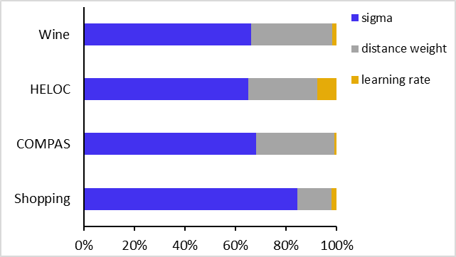
\includegraphics[width=\linewidth]{images/hparams_importance.png}
  \caption{Hyperparameter importance for each dataset. This data was collected when hyperparameter tuning for DT models by using Mahalanobis distance was run. Note that DT models do not use temperature hyperparameters, thus there are only three hyperparameters tuned for those models.}
  \label{fig:hparams importance}
 \end{minipage}
\end{figure}

Empirically, this study found that the quality of the approximation of the original model $f$ has a significant effect on the results. For instance, the number of counterfactual explanations found can range from 20\% to 100\% based on the chosen hyperparameters as demonstrated in Figure \ref{fig:cfe-hist}.
The analysis of the hyperparameter importance for DT models, as presented in Figure \ref{fig:hparams importance}, indicates that the approximation of node activation (sigma) has a strong effect on both the mean Mahalanobis distance and the number of counterfactual explanations found on all datasets. Conversely, changes to the prediction loss-distance loss trade-off parameter (distance weight) and the learning rate of Adam did not exhibit a significant impact on the results. These findings are limited to DT models, and future studies could extend these findings to other model types.

\subsubsection{Model size consideration}
\label{sec:model size}
This study encountered difficulties in running RF models for more than half of the experiments. Initially, it was suspected that this difficulty was caused mainly due to limited computational resources. Also, the original paper's experiments were conducted on a machine with a 48-core CPU and 256GB of RAM, while this study's experiments were conducted on a computer with a quad-core CPU and 8GB of RAM.\\
However, Table \ref{table:model size} in Appendix \ref{appendix:model size comparison} shows that the majority of the retrained models are smaller in size on the disk than the original ones. Despite this, the study was unable to run the retrained models but was able to run the original ones. This suggests that the inability to execute the retrained models may not be solely attributed to their size, and other factors may be contributing.

\section{Discussion}
This study aimed to assess the reliability and effectiveness claims of FOCUS and has drawn several conclusions based on the results of two experiments.\\
Firstly, in regards to the \textit{reliability} claim, the experiments' results validate the original paper's results. Also, the additional experiment demonstrated that FOCUS is robust and generalisable. The additional experiment was limited to DT models, however, future studies could expand the investigation to other tree-based models such as XGBoost \cite{Chen:2016:XST:2939672.2939785} and LightGBM \cite{ke2017lightgbm}.\\
Moreover, this study sheds light on the impact of hyperparameters on the results of FOCUS. It was demonstrated that the selection of hyperparameters can significantly influence the ability of FOCUS to generate counterfactual explanations, thus emphasising the importance of hyperparameter tuning in future studies.\\
Additionally, the study also highlighted the issue of running larger models as described in Section \ref{sec: results beyond original paper}. This study suggests that this difficulty may not be solely due to model size, but other factors may also be contributing. Further research is needed to investigate these factors and find ways to overcome these challenges, to enable the application of FOCUS on larger models.\\
The effectiveness claim is partially supported by this study. While FOCUS was able to generate the counterfactual explanations for all instances, the mean Mahalanobis distances were not consistent with the results reported in the original paper. This deviation raises questions about the reproducibility of the results and highlights the need for further investigation to determine the cause.

% Give your judgement on if your experimental results support the claims of the paper. Discuss the strengths and weaknesses of your approach - perhaps you didn't have time to run all the experiments, or perhaps you did additional experiments that further strengthened the claims in the paper.

\subsection{What was easy}
The original paper's implementation is accessible on GitHub. The repository includes the models and data utilised in the experiments. The authors have also made available a technical appendix, which can be requested and provides all the necessary information, including hyperparameters to reproduce the experiments.

% The implementation of the original paper is publicly available on GitHub. The repository contains the models and data used in the original experiments. Also, the authors provided a technical appendix, which includes all the hyperparameters that were used for the experiments for reproduction upon request. 

% Give your judgement of what was easy to reproduce. Perhaps the author's code is clearly written and easy to run, so it was easy to verify the majority of original claims. Or, the explanation in the paper was really easy to follow and put into code. 

% Be careful not to give sweeping generalizations. Something that is easy for you might be difficult to others. Put what was easy in context and explain why it was easy (e.g. code had extensive API documentation and a lot of examples that matched experiments in papers). 

\subsection{What was difficult}
The code for the implementation was available, however, it utilises outdated packages and the code structure is complex, making it difficult to follow the code. Additionally, the comments and documentation within the code are minimal or absent. Adding unit tests to the codebase helped me to improve my understanding of the structure. Furthermore, for stronger support on the claims made in the paper, it would have been beneficial to run the previously developed framework, DACE, however, due to time constraints and the complexity of using the CPLEX Optimizer \footnote{http://www.ibm.com/analytics/cplex-optimizer}, this study was unable to do so.

% List part of the reproduction study that took more time than you anticipated or you felt were difficult. 

% Be careful to put your discussion in context. For example, don't say "the maths was difficult to follow", say "the math requires advanced knowledge of calculus to follow". 

\subsection{Communication with original authors}
I contacted the authors to obtain the hyperparameters used in the experiments, and they responded promptly with a detailed technical appendix of the original paper.

% Document the extent of (or lack of) communication with the original authors. To make sure the reproducibility report is a fair assessment of the original research we recommend getting in touch with the original authors. You can ask authors specific questions, or if you don't have any questions you can send them the full report to get their feedback before it gets published. 
